%!TEX ROOT=formularioMatematica.tex

\section{Numeri complessi}\label{sec:complex}
Fino ad adesso abbiamo sempre lavorato con numeri appartenenti ad $\mathbb{R}$ al di pi�. Ci sono per�
alcune operazioni che non sono possibili da fare in questo insieme numerico. Una di queste �
\begin{equation*}
\sqrt{-r}\qquad\forall r\in\mathbb{R}^+
\end{equation*}
oppure
\begin{equation*}
\log(n)\qquad \forall n\in\mathbb{R}^-
\end{equation*}
Per sopperire a questa mancanza, � stata introdotta l'unit� immaginaria $i$ che � definita come
\begin{equation*}
i=\sqrt{-1}
\end{equation*}
Un numero complesso � un numero composto da una parte reale e una immaginaria. Esso pu� essere scritto
come
\begin{equation*}
z = \overbrace{a}^{\text{Reale}} + \overbrace{ib}^{\text{Immaginaria}}
\end{equation*}
Quindi
\begin{equation*}
\Re(z) = a \quad\text{e}\quad\Im(z)=ib
\end{equation*}
Questo non � l'unico modo di identificare un numero complesso. Pi� avanti vedremo anche gli altri.\\
$\mathbb{C}$ � quindi definito come
\begin{equation*}
\mathbb{C}=\left\{a+ib: a,b\in\mathbb{R}\right\}
\end{equation*}
Il numero complesso $\bar{z}$ � definito il \textit{coniugato} di $z$ quindi
\begin{equation*}
z=a+ib\qquad\text{e}\qquad\bar{z}=a-ib
\end{equation*}
Si noti che se si deve fare ricorso a \hyperref[ruffini]{Ruffini} si ricerchi lo zero anche in 
$\mathbb{C}$.\\
Per gli esercizi si vada \hyperref[ex:complex]{qui}.

\subsection{Rappresentazione cartesiana}\label{subsec:complex:cart}
Essendo questo numero composto da parte reale e immaginaria, il piano cartesiano non basta pi�. Quindi 
si � deciso di estenderlo a quello che viene comunemente denominato il piano di \textbf{Argrand-Gauss}.
Esso � composto dall'asse delle ascisse come parte reale e quello delle ordinate come parte 
immaginaria.

\begin{center}
	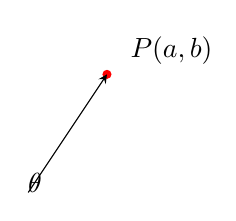
\begin{tikzpicture}
		\coordinate (A) at (1,1.5);
		\coordinate (O) at (0,0);
		\coordinate (B) at (2,0);
		
		\tkzInit[xmin=-2,ymin=-2,xmax=2,ymax=2]
		\tkzGrid
		\tkzAxeXY
		\filldraw[red] (A) circle (0.05);
		\draw[-stealth] (O) -- (A);
		\markangle{O}{A}{B}{0.5}{1.5}{$\theta$}
		\node[above right] at (A) {$P(a,b)$};
	\end{tikzpicture}
\end{center}

La distanza $\overline{OP}$ � detta \emph{modulo} del numero immaginario ed � descritto come
\begin{equation*}
\rho=\norm{z} = \sqrt{a^2+b^2}
\end{equation*}

\subsection{Operazioni tra numeri complessi}
\subsubsection{Somma}
La somma tra due numeri complessi richiede solo di sommare le parti simili fra di loro.
\begin{align*}
&z_1=a_1+i+b_1\qquad\text{e}\qquad z_2=a_2+i_b2
\intertext{La loro somma �}
&z=z_1+z_2=a_1+a_2+i(b_1+b_2)
\end{align*}
Nella somma vige la seguente caratteristica
\begin{equation*}
\overline{z_1+z_2} = \overline{z_1}+\overline{z_2}
\end{equation*}

\subsubsection{Differenza}
La differenza � esattamente come la somma, ovvero si opera parte a parte.
\begin{align*}
&z_1=a_1+i+b_1\qquad\text{e}\qquad z_2=a_2+i_b2
\intertext{La loro differenza �}
&z=z_1-z_2=a_1-a_2+i(b_1-b_2)
\end{align*}
Nella somma e differenza vigono le seguenti caratteristiche
\begin{equation*}
z+\overline{z}=2a\qquad\text{e}\qquad z-\overline{z}=2ib
\end{equation*}

\subsubsection{Prodotto}
Il prodotto si effettua moltiplicando fra di loro parti simili.
\begin{align*}
&z_1=a_1+i+b_1\qquad\text{e}\qquad z_2=a_2+i_b2
\intertext{Il loro prodotto �}
&z=z_1\cdot z_2=a_1a_2-b_1b_2+i(b_1a_2+a_1b_2)
\end{align*}	

\subsubsection{Quoziente}
Il quoziente � un'operazione particolare.
\begin{align*}
&z_1=a_1+i+b_1\qquad\text{e}\qquad z_2=a_2+i_b2
\intertext{Il loro quoziente �}
&z=\frac{z_1}{z_2}=\frac{a_1a_2+b_1b_2}{a_2^2+b_2^2}+i\frac{b_1a_2-a_2b_2}{a_2^2+b_2^2}
\end{align*}

\subsection{Rappresentazione trigonometrica di un numero complesso}
Un modo per definire un numero complesso � gi� stato chiarito. Ne esiste un altro per� che fa capo
alla rappresentazione polare del numero (tramite un altro sistema di assi che identifica un punto
tramite l'angolo che compie un segmento dall'asse $x$).
\begin{equation*}
z=\rho(\cos\theta+i\sin\theta)
\end{equation*}
dove $\theta$ rappresenta l'angolo indicato nella sottosezione
\hyperref[subsec:complex:cart]{Rappresentazione cartesiana}.

\subsubsection{Prodotto}
\begin{align*}
&z_1=\rho_1(\cos\theta_1+i\sin\theta_1)\quad\text{e}\quad z_2=\rho_2(\cos\theta_2+i\sin\theta_2)
\intertext{Il loro prodotto �}
&z=z_1\cdot z_2=\rho_1\rho_2[\cos(\theta_1+\theta_2)_i\sin(\theta_1+\theta_2)]
\end{align*}
\subsubsection{Quoziente}
\begin{align*}
&z_1=\rho_1(\cos\theta_1+i\sin\theta_1)\quad\text{e}\quad z_2=\rho_2(\cos\theta_2+i\sin\theta_2)
\intertext{Il loro quoziente �}
&z=\frac{z_1}{z_2}=\frac{\rho_1}{\rho_2}[\cos(\theta_1-\theta_2)_i\sin(\theta_1-\theta_2)]
\end{align*}

\subsection{Elevazione a potenza}
Messa successivamente alle altre operazioni perch� varia in base alla notazione scelta.
\subsubsection{Algebrica}
\begin{equation*}
z^n = (a+ib)^n
\end{equation*}
\subsubsection{Trigonometrica (Formula di De Moivre)}
\begin{equation*}
z^n=\rho^n(\cos n\theta+i\sin n\theta)
\end{equation*}

\subsection{Radici di un numero complesso}
\begin{align*}
&z = \rho(\cos\theta+i\sin\theta)
\intertext{La radice $n$-esima � pari a}
&\sqrt[n]{z}=\sqrt[n]{\rho}\left(\cos\frac{\theta+2k\pi}{n}+i\sin\frac{\theta+2k\pi}{n}\right)
\end{align*}
Una caratteristica interessante delle radici � la loro rappresentazione grafica. Infatti se si prendono
le coordinate e si uniscono fra di loro si costruir� un poligono regolare con $n$ lati inscritto 
all'interno di una circonferenza di raggio $\rho$.\\
Per calcolarle, sostituire $k$ con i numeri che vanno da $0$ a $n-1$.

\subsection{Teroema fondamentale dell'algebra}
Esso cita:
\begin{tfa}
	Ogni polinomio di grado $n\geq1$
	\begin{equation*}
	P(x) = \sum\limits_{i=0}^{n} a_ix^i
	\end{equation*}
	a coefficienti $\mathbb{C}$ ha almeno uno zero in $\mathbb{C}$.
\end{tfa}
Da questo deriva
\begin{tfa-ext}\hypertarget{teor:tfa-ext}{}
	Per ogni polinomio di grado $n\geq1$
	\begin{equation*}
	P(x) = \sum\limits_{i=0}^{n} a_ix^i
	\end{equation*}
	a coefficienti $\mathbb{C}$ ha esattamente $n$ zeri in $\mathbb{C}$, con la convenzione di contare
	$r$ volte uno zero di molteplicit� $r$.
\end{tfa-ext}
Per molteplicit� si intende
\begin{molteplic}
	Se il polinomio $P(x)$ si pu� scomporre nel prodotto
	\begin{equation*}
	P(x) = (x-\alpha)^rP_r(x)
	\end{equation*}
	dove il polinomio $P_r(x)$ � di grado $(n-r)$, si dice che $P(x)$ � divisibile per $(x-\alpha)^r$
	e se $P_r(x)$ non � divisibile per $(x-\alpha)$, si dice che $\alpha$ � uno \textbf{zero di 
	molteplicit�} $r$ per $P(x)$.
\end{molteplic}

\subsection{Esponenziali complessi}
Detta $e$ la costante di Nepero (anche chiamato numero di Eulero)
\begin{equation*}
e \approx 2.71828\ldots
\end{equation*}
si definisce per ogni numero complesso $z = a+ib$ l'esponenziale complesso $e^{a+ib}$ come il numero
complesso 
\begin{equation*}
w=e^x(\cos a+i\sin b)
\end{equation*}
Quindi possiamo dire che 
\begin{equation*}
e^{z} = \rho e^{i\theta}
\end{equation*}
Proprio da questa formula ne viene ricavata una delle pi� famose della storia della matematica
\begin{equation*}
e^{i\pi}+1=0
\end{equation*}
che collega 5 unit� fondamentali della matematica.

\subsection{Formule di Eulero}
\begin{equation*}
\cos\theta=\frac{e^{i\theta}+e^{-i\theta}}{2}\qquad\sin\theta=\frac{e^{i\theta}-e^{-i\theta}}{2}
\end{equation*}
Queste formule permettono di trasferire tutte le caratteristiche della notazione trigonometrica in 
quella esponenziale.